\documentclass[tikz]{standalone}
\usepackage{amsmath}
\usetikzlibrary{arrows.meta,backgrounds,calc,fit}

\begin{document}
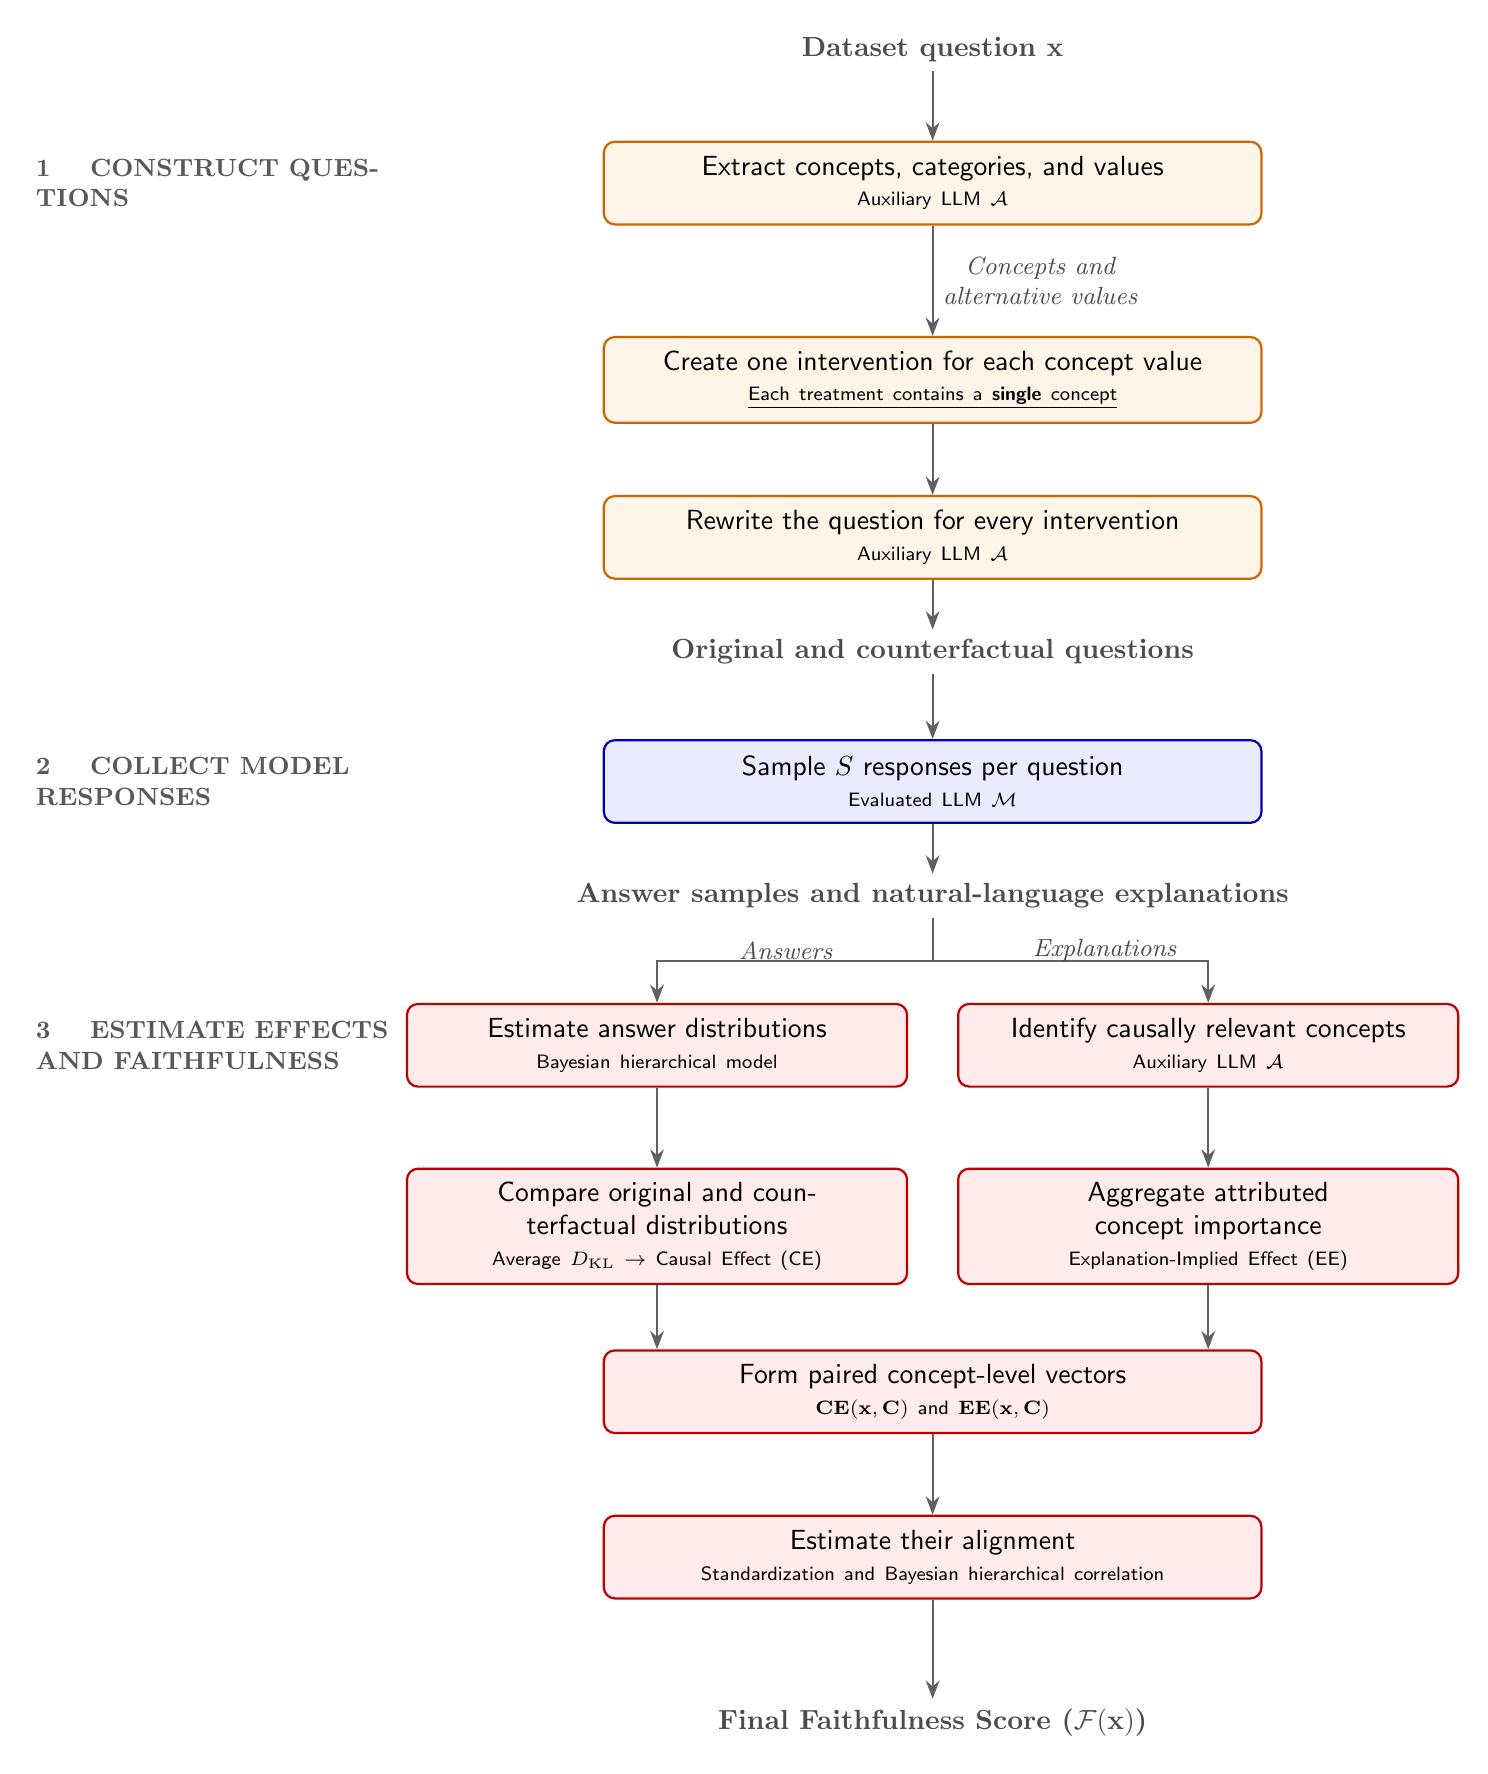
\begin{tikzpicture}[
    font=\sffamily,
    flow/.style={->, >=Stealth, thick, draw=gray!75!black},
    % Size styles
    node wide/.style={rounded corners, align=center, text width=8cm, minimum height=1.05cm, thick, inner sep=5pt},
    node branch/.style={rounded corners, align=center, text width=6cm, minimum height=1.05cm, thick, inner sep=5pt},
    % Color styles based on phase
    phase1/.style={draw=orange!80!black, fill=orange!9},
    phase2/.style={draw=blue!70!black, fill=blue!8},
    phase3/.style={draw=red!75!black, fill=red!8},
    % Other styles
    phaseTitle/.style={font=\bfseries\small, text=gray!70!black, fill=white, inner sep=3pt, text width=4.5cm, align=left},
    data/.style={font=\small\itshape, align=center, text=black!70}
]

\node[data, font=\bfseries] (input) at (0,0) {Dataset question $\mathbf{x}$};

% --- PHASE 1 (Orange) ---
\node[node wide, phase1] (extract) at (0,-1.7) {Extract concepts, categories, and values\\[-1pt] \scriptsize Auxiliary LLM $\mathcal{A}$};
\draw[flow] (input) -- (extract);
\node[node wide, phase1] (interventions) at (0,-4.2) {Create one intervention for each concept value\\[-1pt] \scriptsize \underline{Each treatment contains a \textbf{single} concept}};
\draw[flow] (extract) -- node[data, right] {Concepts and\\alternative values} (interventions);
\node[node wide, phase1] (rewrite) at (0,-6.2) {Rewrite the question for every intervention\\[-1pt] \scriptsize Auxiliary LLM $\mathcal{A}$};
\draw[flow] (interventions) -- (rewrite);
\node[data, font=\bfseries] (questions) at (0,-7.65) {Original and counterfactual questions};
\draw[flow] (rewrite) -- (questions);

\node[phaseTitle, anchor=west] at (-11.5,-1.7) {1 \quad CONSTRUCT QUESTIONS};

% --- PHASE 2 (Blue) ---
\node[node wide, phase2] (sample) at (0,-9.3) {Sample $S$ responses per question\\[-1pt] \scriptsize Evaluated LLM $\mathcal{M}$};
\draw[flow] (questions) -- (sample);
\node[data, font=\bfseries] (observations) at (0,-10.75) {Answer samples and natural-language explanations};
\draw[flow] (sample) -- (observations);

\node[phaseTitle, anchor=west] at (-11.5,-9.3) {2 \quad COLLECT MODEL RESPONSES};

% --- PHASE 3 (Red) ---
\node[node branch, phase3] (probability) at (-3.5,-12.65) {Estimate answer distributions\\[-1pt] \scriptsize Bayesian hierarchical model};
\node[node branch, phase3] (mentions) at (3.5,-12.65) {Identify causally relevant concepts\\[-1pt] \scriptsize Auxiliary LLM $\mathcal{A}$};
\draw[flow] (observations.south) -- ++(0,-0.55) -| (mentions.north);
\draw[flow] (observations.south) -- ++(0,-0.55) -| (probability.north);
\node[data, anchor=east] at (-1.15,-11.45) {Answers};
\node[data, anchor=west] at (1.15,-11.45) {Explanations};

\node[node branch, phase3] (ce) at (-3.5,-14.95) {Compare original and counterfactual distributions\\[-1pt] \scriptsize Average $D_{\mathrm{KL}}$ $\rightarrow$ Causal Effect (CE)};
\node[node branch, phase3] (ee) at (3.5,-14.95) {Aggregate attributed concept importance\\[-1pt] \scriptsize Explanation-Implied Effect (EE)};
\draw[flow] (mentions) -- (ee);
\draw[flow] (probability) -- (ce);

\node[node wide, phase3] (vectors) at (0,-17.05) {Form paired concept-level vectors\\[-1pt] \scriptsize $\mathbf{CE}(\mathbf{x},\mathbf{C})$ and $\mathbf{EE}(\mathbf{x},\mathbf{C})$};

\draw[flow] (ee.south) -- (ee.south |- vectors.north);
\draw[flow] (ce.south) -- (ce.south |- vectors.north);

\node[node wide, phase3] (correlation) at (0,-19.15) {Estimate their alignment\\[-1pt] \scriptsize Standardization and Bayesian hierarchical correlation};
\draw[flow] (vectors) -- (correlation);
\node[data, font=\bfseries] (final) at (0,-21.25) {Final Faithfulness Score ($\mathcal{F}(\mathbf{x})$)};
\draw[flow] (correlation) -- (final.north);

\node[phaseTitle, anchor=west] at (-11.5,-12.65) {3 \quad ESTIMATE EFFECTS AND FAITHFULNESS};

\end{tikzpicture}
\end{document}
